\section{Auswertung}
\subsection{Fehlerrechnung}
In der folgenden Auswertung werden Mittelwerte mit
\begin{equation}
\bar{x} = \frac{1}{N} \sum_{\mathclap{i=1}}^N x_{\text{i}}
\label{eqn:mittelwert}
\end{equation}
und der zugehörige Fehler mit 
\begin{equation}
\Delta\bar{x} = \frac{1}{\sqrt{N}} \sqrt{\frac{1}{N-1}\sum_{\mathclap{i=1}}^N (x_{\text{i}}-\bar{x})^2}
\label{eqn:mittelwertfehler}
\end{equation}
berechnet. 
Beim Rechnen mit mehreren fehlerbehafteten Werten wird die Gauß'sche Fehlerfortpflanzung zur Berechnung des neuen Fehlers genutzt:
\begin{equation}
\Delta{f} = \sqrt{\sum_{i=1}^{N} \biggl(\frac{\delta{f}}{\delta{x}_{\text{i}}}\biggr)^2 \cdot (\Delta{x_{\text{i}}})^2}.
\label{eqn:gauss}
\end{equation}
\subsection{Bestimmung der Apparatekonstanten}
Um später die Viskosität von Wasser bei verschiedenen Temperaturen berechnen zu können, muss die Apparatekonstante $K_{\text{gr}}$ der großen Kugel bestimmt werden.
Hierfür werden zunächst die Dichten der beiden Kugeln aus den gegebenen Massen
\begin{equation*}
\begin{aligned}
m_{\text{kl}} &= 4{,}48 \cdot10^{-3} \symup{kg} \\
m_{\text{gr}} &= 4{,}97 \cdot 10^{-3}\symup{kg}
\end{aligned}
\end{equation*}
sowie den Radien der Kugeln aus Tabelle \eqref{tab:radienkugel} berechnet.

\begin{table}[htbp]
\centering
\caption{Radien der Kugeln}
\label{tab:radienkugel}
\begin{tabular}{
S[table-format=1.5, table-auto-round] 
S[table-format=1.5, table-auto-round]
}
\toprule
{Kleine Kugel} & {Große Kugel}  \\
{$r_{\text{kl}}$/$10^{-3}$m} & {$r_{\text{gr}}$/$10^{-3}$m} \\
\midrule
7.7545 & 7.763 \\
7.7545 & 7.7625  \\
7.75425 & 7.76275  \\
7.75425 & 7.76275 \\
7.75475 & 7.76325  \\
\bottomrule
\end{tabular}
\end{table}
Der Mittelwert der Radien wird mit Gleichung \eqref{eqn:mittelwert} und der Fehler des Mittelwerts mit Gleichung \eqref{eqn:mittelwertfehler} zu

\begin{equation*}
\begin{aligned}
r_{\text{kl}} &= (7{,}75445 \pm 0{,}00009) \cdot 10^{-3}\symup{m} \\
r_{\text{gr}} &= (7{,}76285 \pm 0{,}00013) \cdot 10^{-3}\symup{m}
\end{aligned}
\end{equation*}
berechnet. Die Volumina der Kugeln mit zugehörigem Fehler können dann mit Gleichung \eqref{eqn:gauss} errechnet werden. Es ergibt sich:
\begin{equation*}
\begin{aligned}
V_{\text{kl}} &= (1{,}95318 \pm 0{,}00007) \cdot 10^{-6}\symup{m^3} \\
V_{\text{gr}} &= (1{,}95953 \pm 0{,}00009) \cdot 10^{-6}\symup{m^3}
\end{aligned}
\end{equation*}
Hieraus können nun die Dichten der beiden Kugeln berechnet werden. Wieder wird Gleichung \eqref{eqn:gauss} für die Berechnung des Fehlerwertes genutzt.
\begin{equation*}
\begin{aligned}
\rho_{\text{kl}} &= (2293{,}65 \pm 0{,}08)\, \symup{\frac{kg}{m^3}} \\
\rho_{\text{gr}} &= (2536{,}321 \pm 0{,}116)\, \symup{\frac{kg}{m^3}}
\end{aligned}
\end{equation*}
 
Weiterhin wird für die Berechnung der Apparatekonstanten die Viskosität $\eta_{\text{RT}}$ von Wasser bei Raumtemperatur bestimmt. Verwendet werden
\begin{equation*}
\begin{aligned}
K_{\text{kl}} &= 7{,}64 \cdot 10^{-8}\, \symup{\frac{Pa \cdot m^3}{kg}} \\
\rho_{\text{fl}} &= 998{,}2 \, \symup{\frac{kg}{m^3}}
\end{aligned}
\end{equation*}
wobei $K_{\text{kl}}$ die bereits gegebene Apparatekonstante der kleinen Kugel ist und $\rho_{\text{fl}}$ die Dichte von Wasser bei Raumtemperatur \cite{waterdensity}.
Zudem entnimmt man die Fallzeiten der beiden Kugeln von
\begin{equation*}
\begin{aligned}
t_{\text{kl}} &= (12{,}42 \pm 0{,}09)\, \symup{s} \\
t_{\text{gr}} &= (73{,}4 \pm 0{,}3)\, \symup{s} \\
\end{aligned}
\end{equation*}
aus Tabelle \eqref{tab:fallzeitenkugel}.

\begin{table}[htbp]
\centering
\caption{Fallzeiten der Kugeln durch Wasser bei Raumtemperatur}
\label{tab:fallzeitenkugel}
\begin{tabular}{
S[table-format=2.2, table-auto-round] 
S[table-format=2.2, table-auto-round]
}
\toprule
{Kleine Kugel} & {Große Kugel}  \\
{$t_{\text{kl}}$/s} & {$t_{\text{gr}}$/s} \\
\midrule
12.03 & 72.63 \\
12.06 & 72.34 \\
12.24 & 73.27 \\
12.37 & 73.26 \\
12.40 & 74.61 \\
12.95 & 72.85 \\
12.60 & 72.82 \\
12.63 & 73.56 \\
12.44 & 74.28 \\
12.47 & 74.66 \\
\bottomrule
\end{tabular}
\end{table}

Nun lässt sich die Viskosität $\eta_{\text{RT}}$ mit Gleichung [K, DCIHTE; ZEIT] bestimmen. Sie beträgt
\begin{equation*}
\eta_{\text{RT}} = (1{,}23 \pm 0{,}09) \cdot 10^{-3} \symup{Pa \cdot s} \\
\end{equation*}
wobei der Fehlerwert wiederum aus der Gauß'schen Fehlerfortpflanzung \eqref{eqn:gauss} stammt.

Zuletzt wird Gleichung[K; DICHTE; ZEIT] nach $K_{\text{gr}}$ umgestellt. Mit den zuvor errechneten Werten ergibt sich eine Apparatekonstante von
\begin{equation*}
K_{\text{gr}} = (1{,}09 \pm 0{,}08) \cdot 10^{-8} \symup{\frac{Pa \cdot m^3}{kg}} \\
\end{equation*}

\subsection{Bestimmung der Temperaturabhängigkeit der Viskosität}
Wie bei der Bestimmung der Apparatekonstanten $K_{\text{gr}}$ kann Gleichung [K; DICHTE; ZEIT] für die Berechnung der Viskositäten von Wasser bei unterschiedlichen Temperaturen verwendet werden.
Hierbei sind $K_{\text{gr}}$, $\rho_{\text{gr}}$ und $t_{\text{gr}}$ fehlerbehaftete Größen, weshalb die Gauß'sche Fehlerfortpflanzung mit Gleichung \eqref{eqn:gauss} durchgeführt werden muss. 
Für die Dichte $\rho_{\text{fl}}$ von Wasser bei verschiedenen Temperaturen werden Literaturdaten \cite{waterdensity} verwendet.

\begin{table}[htbp]
\centering
\caption{Messdaten zur Bestimmung der Temperaturabhängigkeit der Viskosität von Wasser}
\label{tab:some_data}
\begin{tabular}{
S[table-format=3.2] 
S[table-format=2.2,table-figures-uncertainty=1]
S[table-format=3.2]
S[table-format=1.2, table-figures-uncertainty=1]
}
\toprule
{Temperatur} & {Fallzeit} & {Dichte Wasser} & {Viskosität} \\
{T/K} & {$t_{\text{gr}}$/s} & {$\rho_{\text{fl}}$/$\symup{\frac{kg}{m^3}}$} & {$\eta $/$10^{-3} \symup{Pa \cdot s}$}\\
\midrule
303.15   & 61.76 \pm 1.07 & 995.64 & 6.12 \pm 0.13 \\
307.15   & 55.7 \pm 0.4   & 994.37 & 5.52 \pm 0.08 \\
310.15   & 52.6 \pm 0.2   & 993.32 & 5.22 \pm 0.06 \\
313.20   & 49.5 \pm 0.2   & 992.19 & 4.91 \pm 0.06 \\
317.15   & 47.6 \pm 0.4   & 990.63 & 4.73 \pm 0.07 \\
321.15   & 43.5 \pm 0.1   & 988.93 & 4.33 \pm 0.05 \\
325.65   & 40.7 \pm 0.2   & 986.89 & 4.05 \pm 0.02 \\
329.65   & 37.9 \pm 0.4   & 984.97 & 3.78 \pm 0.06 \\
333.15   & 36.5 \pm 0.3   & 983.20 & 3.64 \pm 0.05 \\
336.15   & 34.9 \pm 0.1   & 981.63 & 3.49 \pm 0.04 \\
\bottomrule
\end{tabular}
\end{table}
Im Folgenden wird der natürliche Logarithmus der Viskosität gegen den Kehrwert der Temperatur aufgetragen, wie in Abbildung \eqref{fig:bildandrade} zu sehen ist. 
\begin{figure}[!h]
\centering
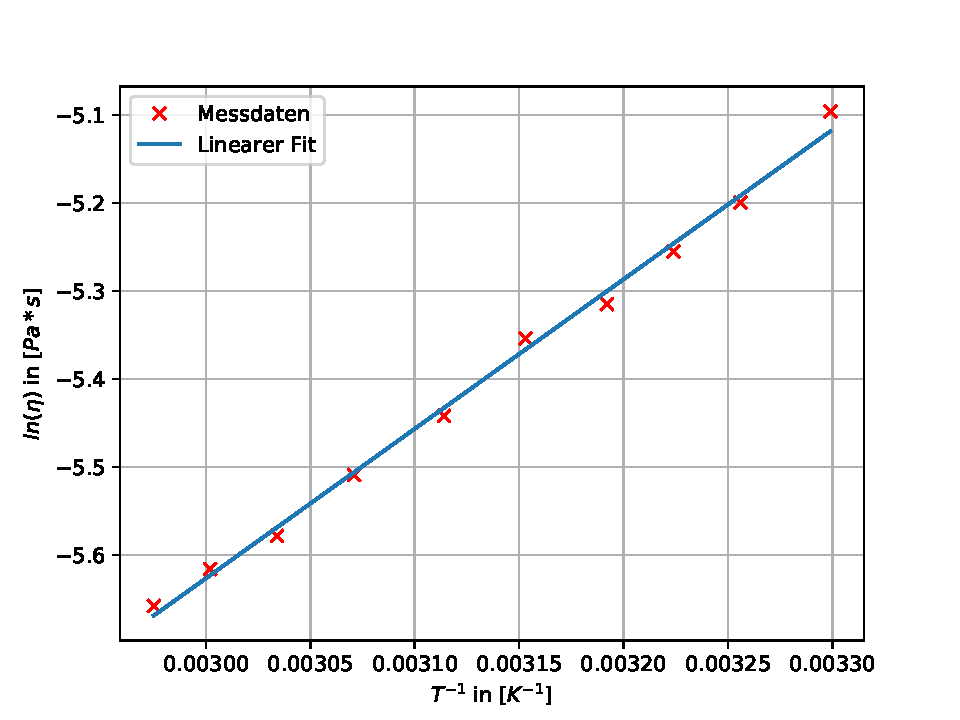
\includegraphics[scale=.9]{Andrade.pdf}
\caption{Bestimmung der Konstanten der Andradeschen Gleichung}
\label{fig:bildandrade}
\end{figure}

Mithilfe des Graphen lassen sich nun die Konstanten der 
Andradeschen Gleichung errechnen:
\begin{equation*}
\begin{aligned}
\eta(T) &= Ae^{\frac{B}{T}} \\
\iff \text{ln}(\eta) &= \text{ln}(A) + \frac{B}{T} \\
A &= (2.2 \pm 0.5)\cdot 10^{-5} \symup{Pa \cdot s} \\
B &= (1698.9 \pm 39.3) \symup{K} \\
\end{aligned}
\end{equation*}

\newpage
Zuletzt wird geprüft, ob die Strömung laminar oder turbulent ist. Hierzu wird die Reynoldszahl $Re_{\text{max}}$ der kleinen und der großen Kugel berechnet und dann mit dem kritischen Wert der 
Reynoldszahl $Re_{\text{krit}}$=1160 verglichen.
Wird in Gleichung [REYNOLDSZAHL] $d=2r_{\text{kl/gr}}$ und $v=\frac{x}{t_{\text{kl/gr}}}$ gesetzt, so ergibt sich
\begin{equation}
\begin{aligned}
Re = \frac{\rho \cdot 2r_{\text{kl/gr}} \cdot x}{\eta \cdot t_{\text{kl/gr}}}
\end{aligned}
\end{equation}
wobei x die Fallstrecke der Kugeln ist und $x=0.1\symup{m}$ \cite[3]{anleitung107} beträgt. Um den maximalen Wert der Reynoldszahl zu erhalten, wird jeweils die kleinste Fallzeit der Kugeln gewählt. Bei der 
großen Kugel entspricht dies der Fallzeit bei der höchsten Wassertemperatur.

Die Reynoldszahlen der beiden Kugel betragen damit
\begin{equation*}
\begin{aligned}
Re_{\text{max,kl}} &= 101.4 \pm 7.5 \\
Re_{\text{max,gr}} &= 12.5 \pm 0.2
\end{aligned}
\end{equation*}

